\documentclass[aspectratio=169,20pt]{beamer}
\usetheme{default}
\usecolortheme{dove}
\geometry{paperwidth=320mm,paperheight=180mm}
\usepackage[T1]{fontenc}
\usepackage{lmodern}
\usepackage{graphicx}
\usepackage{booktabs}
\setbeamertemplate{navigation symbols}{}
\setbeamertemplate{footline}[frame number]
\setbeamersize{text margin left=12mm,text margin right=12mm}
\setbeamerfont{frametitle}{size=\fontsize{28}{33}\selectfont,series=\bfseries}
\setbeamerfont{normal text}{size=\fontsize{20}{25}\selectfont}
\setbeamercolor{normal text}{fg=black,bg=white}
\hypersetup{pdftitle={MIMESIS: Seven-slide project pitch},pdfauthor={Arjun Vijay Prakash},colorlinks=true,urlcolor=black}
\newcommand{\source}[1]{\par\smallskip{\fontsize{13}{16}\selectfont #1\par}}
\begin{document}

\begin{frame}{MIMESIS: choosing Earth terrain for Moon and Mars preparation}
\begin{columns}[T,onlytextwidth]
\begin{column}{.34\textwidth}
\textbf{The challenge}\par
Identify useful Earth analogues and explain where the analogy breaks.
\par\medskip

\textbf{Our solution}\par
Compare NASA terrain measurements, inspect candidate locations and expose choices that depend on the scoring assumptions.
\par\medskip

\textbf{Scope}\par
Regional terrain mapping, with source-linked evidence and GIS exports.
\end{column}
\begin{column}{.63\textwidth}
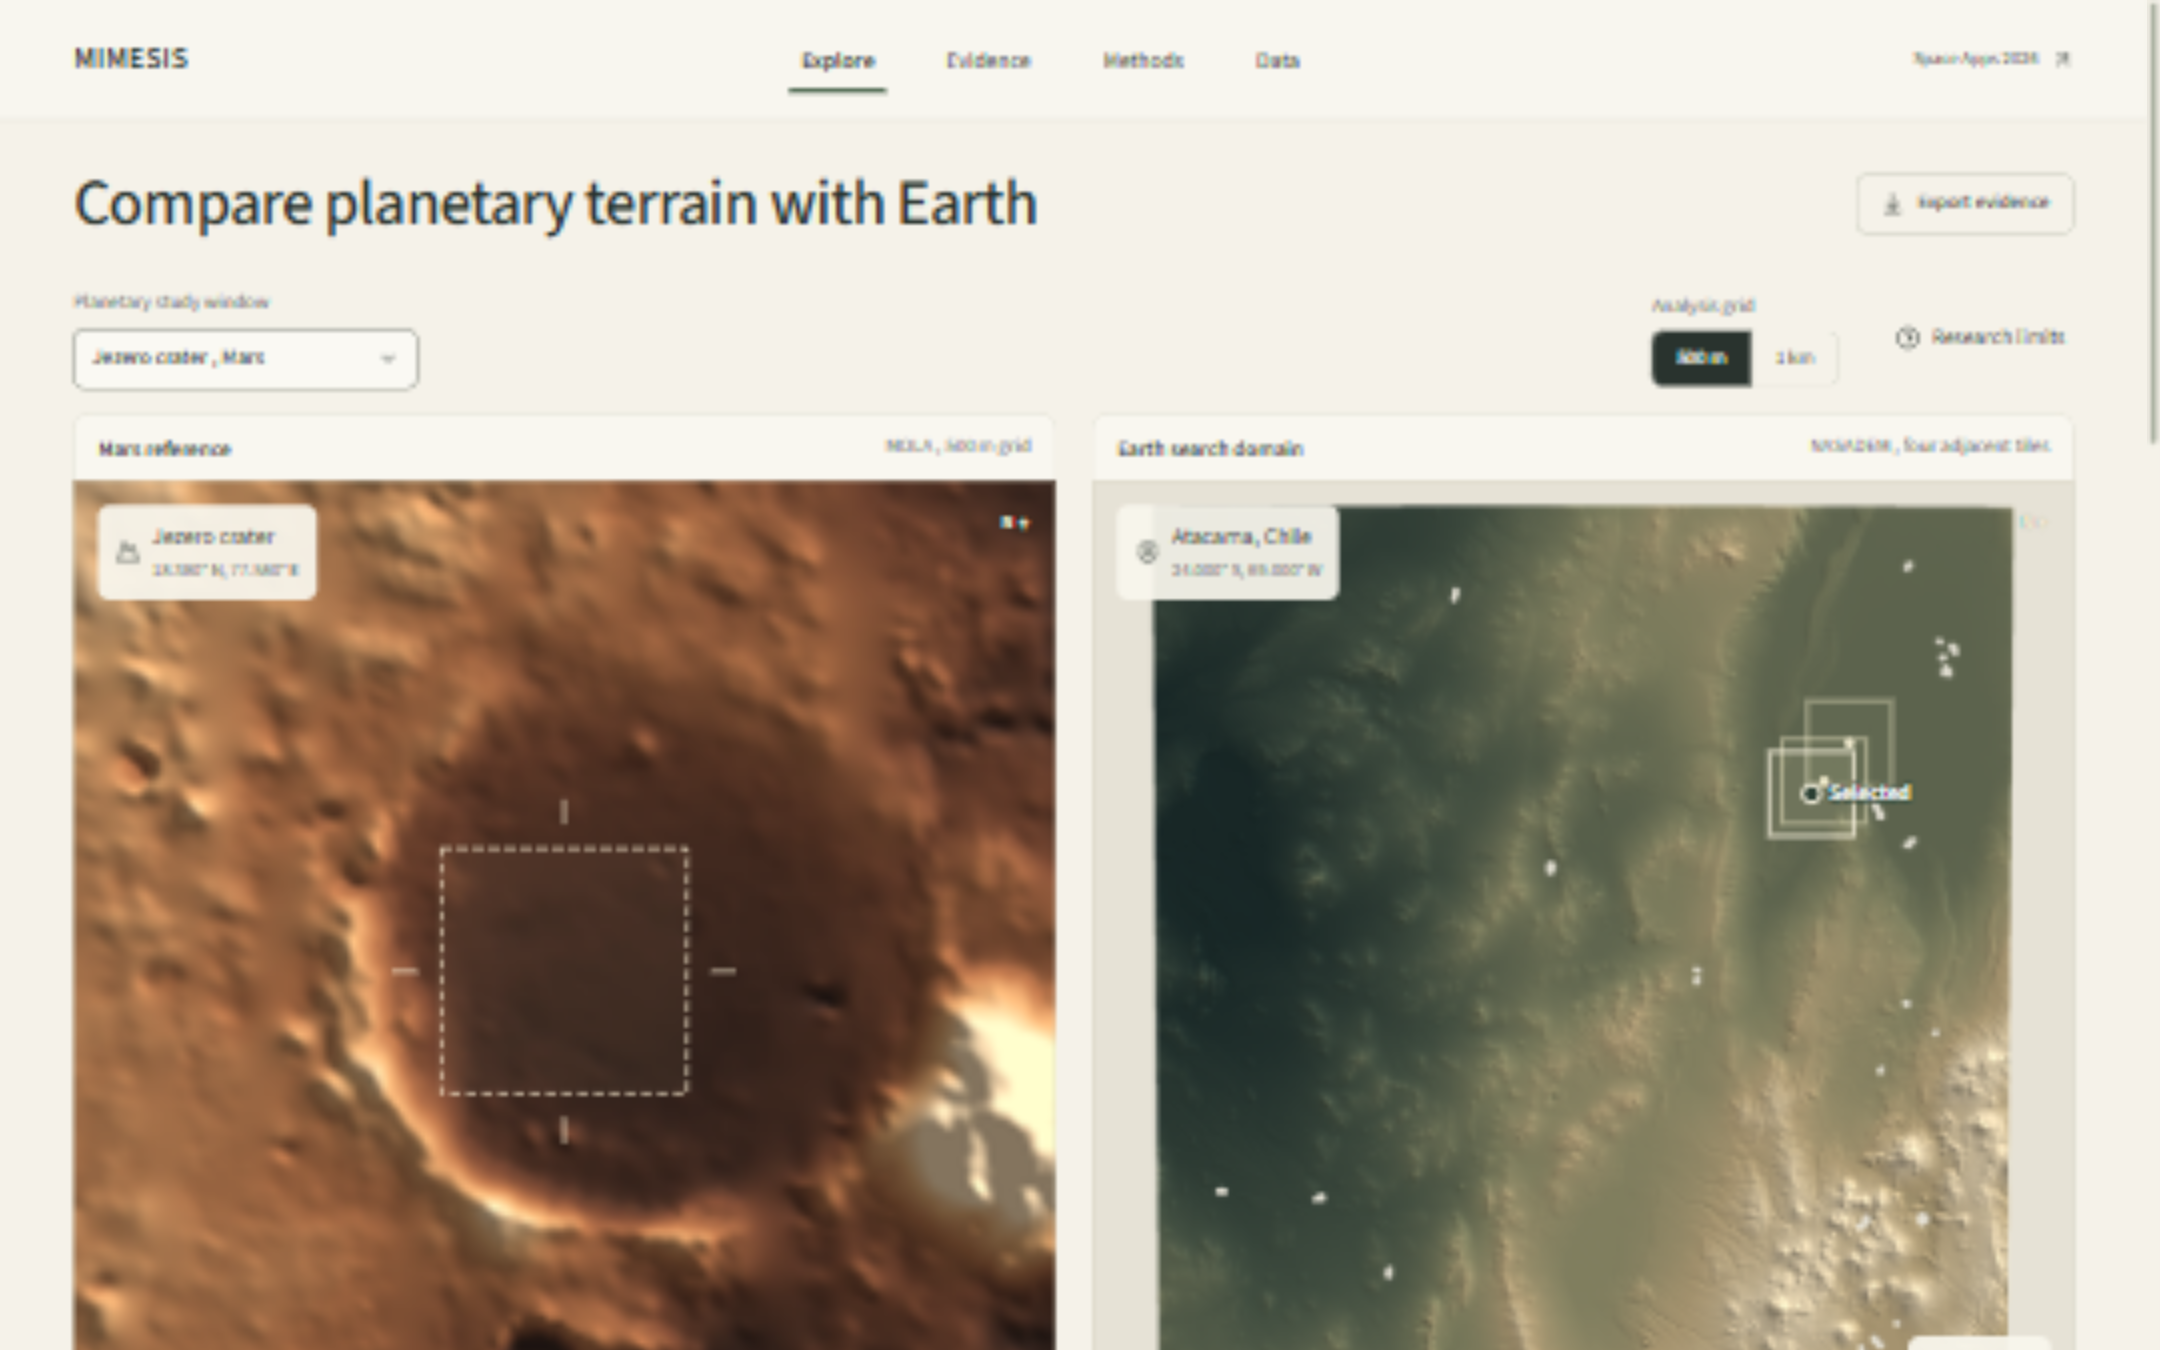
\includegraphics[width=\linewidth,height=112mm,keepaspectratio]{images/explore.png}
\source{Working application: Explore. Elevation-derived views, not satellite photographs.}
\end{column}
\end{columns}
\par\medskip
\source{Arjun Vijay Prakash, Grade XI, City Montessori School, Kanpur Road, Lucknow, India. NASA Space Apps 2026, Lucknow local event.}
\end{frame}

\begin{frame}{NASA observations become explicit comparison contracts}
\begin{columns}[T,onlytextwidth]
\begin{column}{.46\textwidth}
\textbf{Earth: NASADEM}\par
Namib and Atacama; 3,693 overlapping windows.
\par\medskip
\textbf{Mars: MGS MOLA}\par
Jezero, Nili, Isidis and Syrtis.
\par\medskip
\textbf{Moon: LRO LOLA}\par
Taurus--Littrow and Shackleton rim.
\par\medskip
20 km local windows; 80 km context.\par
3 km center spacing; 500 m / 1 km support.
\end{column}
\begin{column}{.49\textwidth}
\textbf{Contract A: four scalar descriptors}\par
Relief, median slope, upper-decile slope and residual roughness. Fixed scales; equal-weight RMS distance.
\par\medskip
\textbf{Contract B: four terrain groups}\par
Slope distributions, relief/position, roughness/organization and context. Maximum loss over 35 scenarios.
\par\medskip
\textbf{Then test the geography}\par
Compare IDs, center displacement, footprint overlap and one-to-one nearby matches.
\end{column}
\end{columns}
\par\medskip
\source{Frozen MIMESIS bundle; source ancestry and baseline provenance in the paper. Analysis spacing is not native resolution; overlapping windows are not independent sites.}
\end{frame}

\begin{frame}{Evidence demo: different ranks can share the same ground}
\begin{columns}[T,onlytextwidth]
\begin{column}{.68\textwidth}
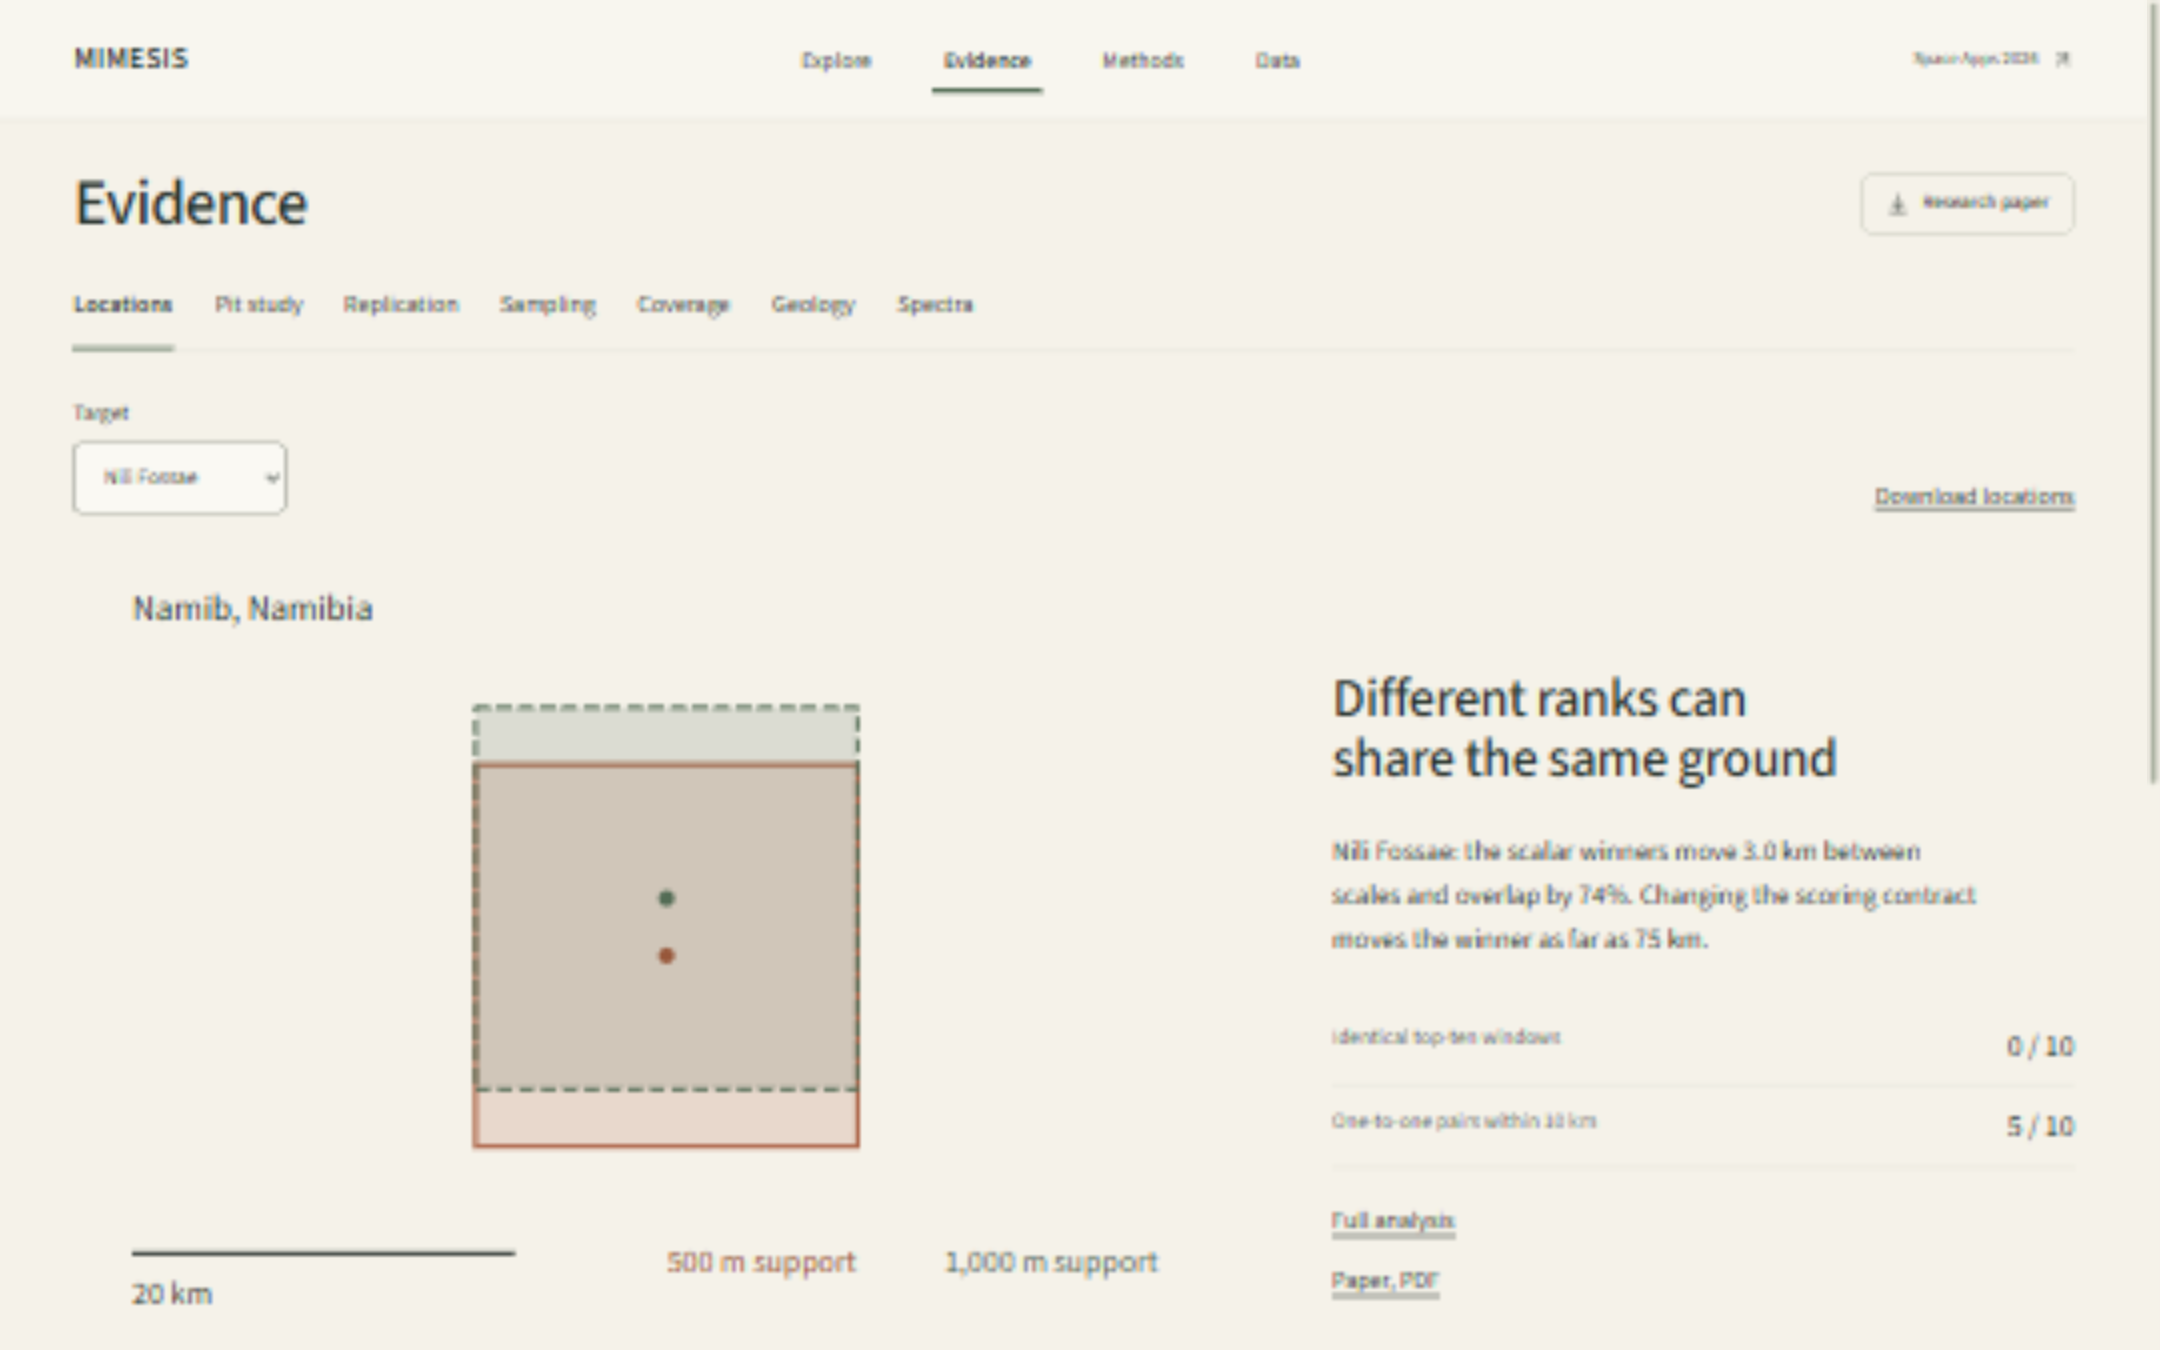
\includegraphics[width=\linewidth,height=127mm,keepaspectratio]{images/evidence.png}
\end{column}
\begin{column}{.29\textwidth}
\textbf{Nili Fossae, scalar contract}
\par\medskip

0 shared top-ten IDs.\par
3 km between winning centers.\par
73.9\% footprint intersection-over-union.
\par\medskip

5 of 10 pairs match one-to-one within 10 km.
\par\medskip

Exact turnover exaggerates geographic replacement here; it does not prove complete stability.
\end{column}
\end{columns}
\source{Actual Evidence screen, Locations tab. Reproduce with scripts/measure\_site\_stability.py. Radius is exploratory, not an operational travel limit.}
\end{frame}

\begin{frame}{Changing the scoring contract can change the continent}
\begin{columns}[T,onlytextwidth]
\begin{column}{.64\textwidth}
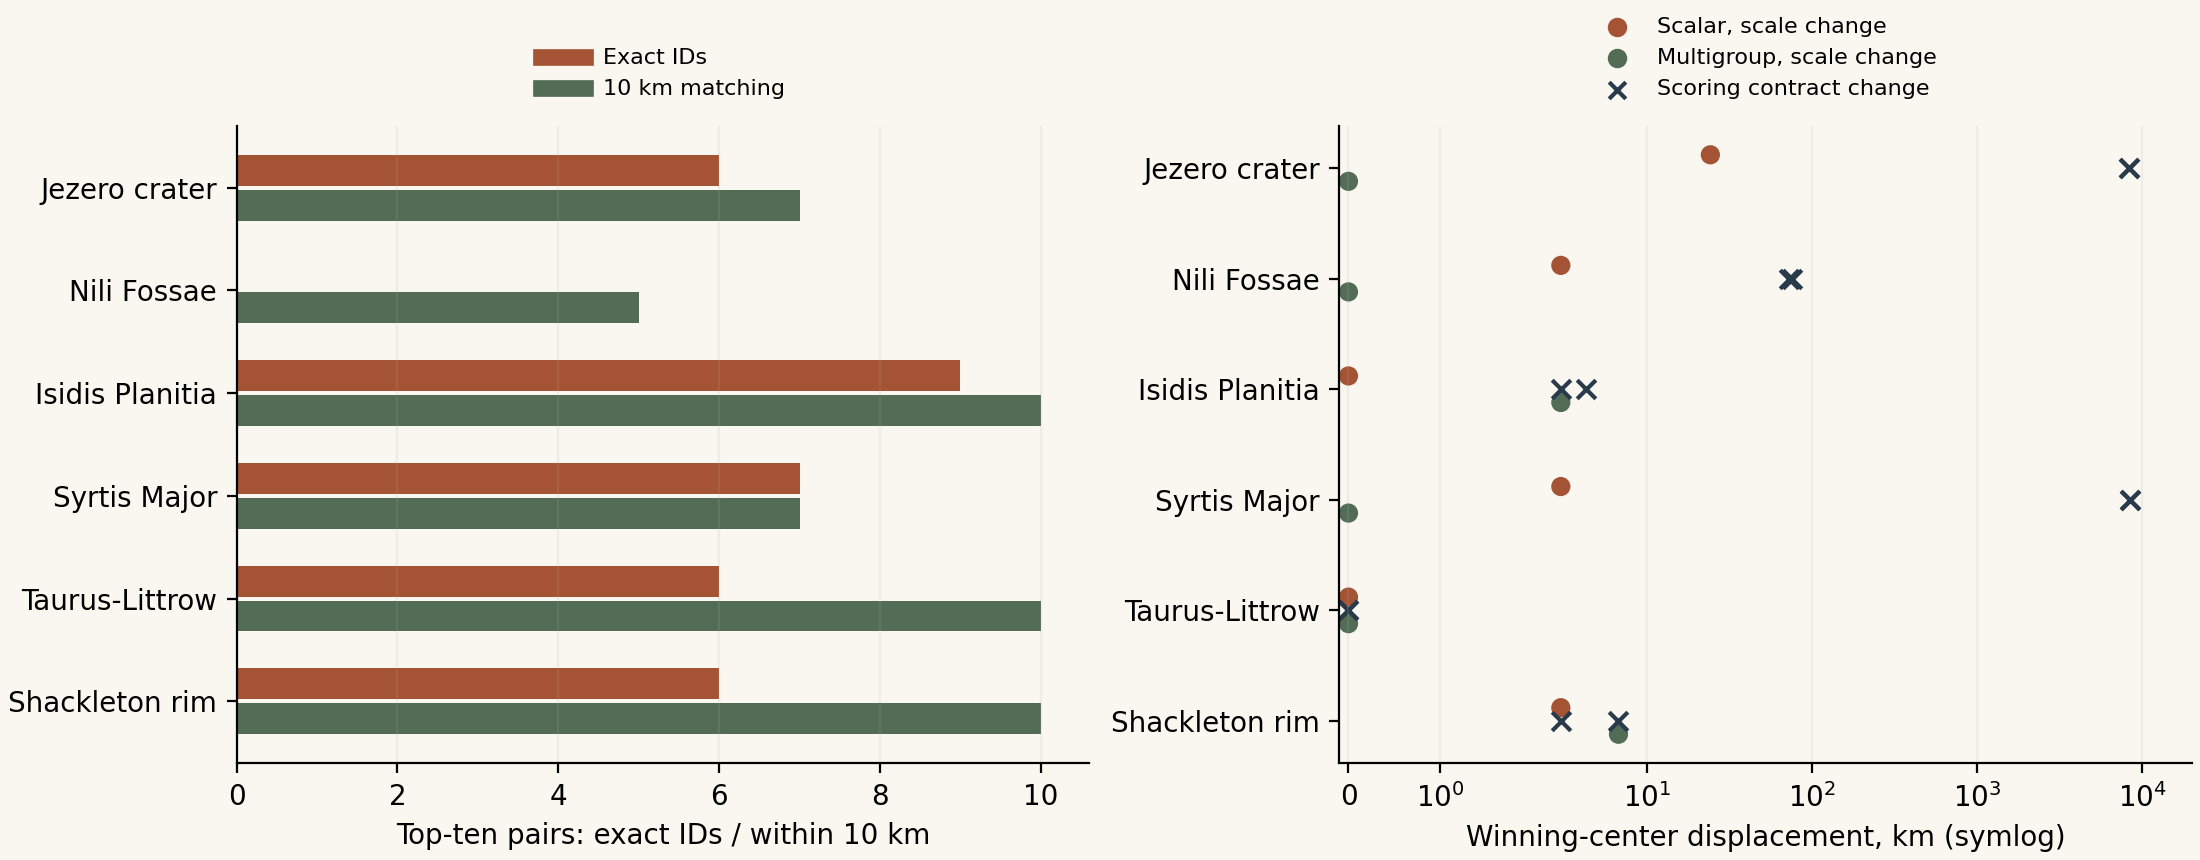
\includegraphics[width=\linewidth]{../paper/site-stability.png}
\par\medskip
\source{Six targets, two contracts and two supports. The chart uses a symmetric-logarithmic distance axis. Conditions are correlated diagnostics.}
\end{column}
\begin{column}{.33\textwidth}
\textbf{Change support within a contract}\par
Largest winner displacement: 24.2 km.
\par\medskip
\textbf{Change the scoring contract}\par
Jezero and Syrtis move between Namibia and Chile: 8,349--8,484 km.
\par\medskip
Agreement at two scales does not establish agreement across assumptions.
\par\medskip
The contracts differ in several ingredients; neither is validated as better.
\end{column}
\end{columns}
\end{frame}

\begin{frame}{Methods and Data make the comparison inspectable}
\begin{columns}[T,onlytextwidth]
\begin{column}{.49\textwidth}
\textbf{Methods}\par
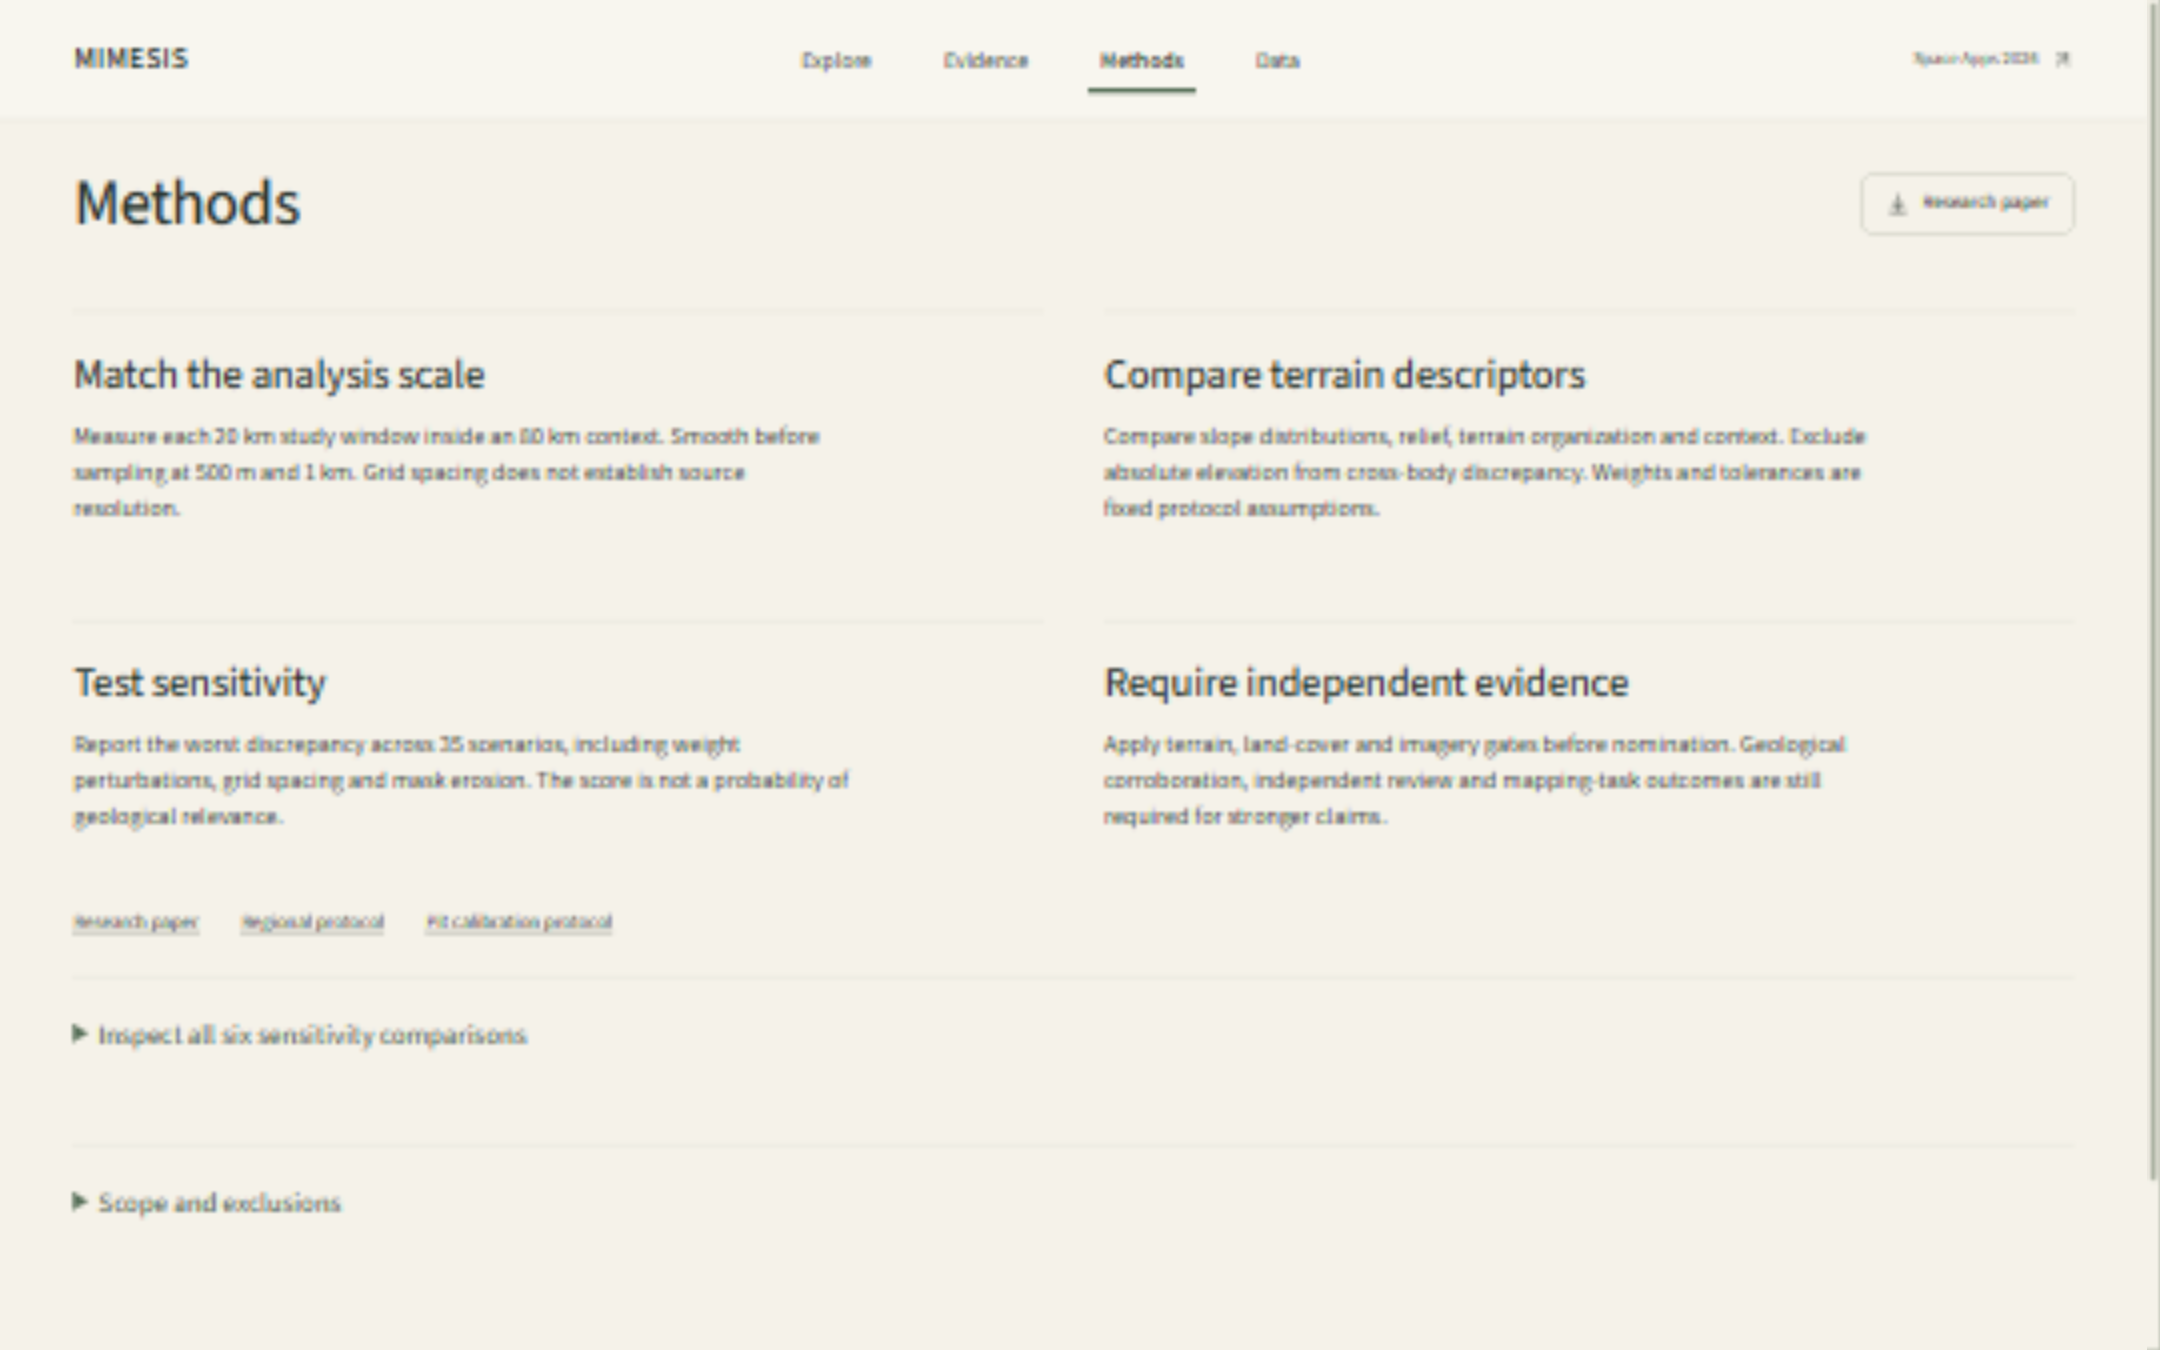
\includegraphics[width=\linewidth,height=104mm,keepaspectratio]{images/methods.png}
\source{Window definition, descriptors, sensitivity and evidence requirements.}
\end{column}
\begin{column}{.49\textwidth}
\textbf{Data}\par
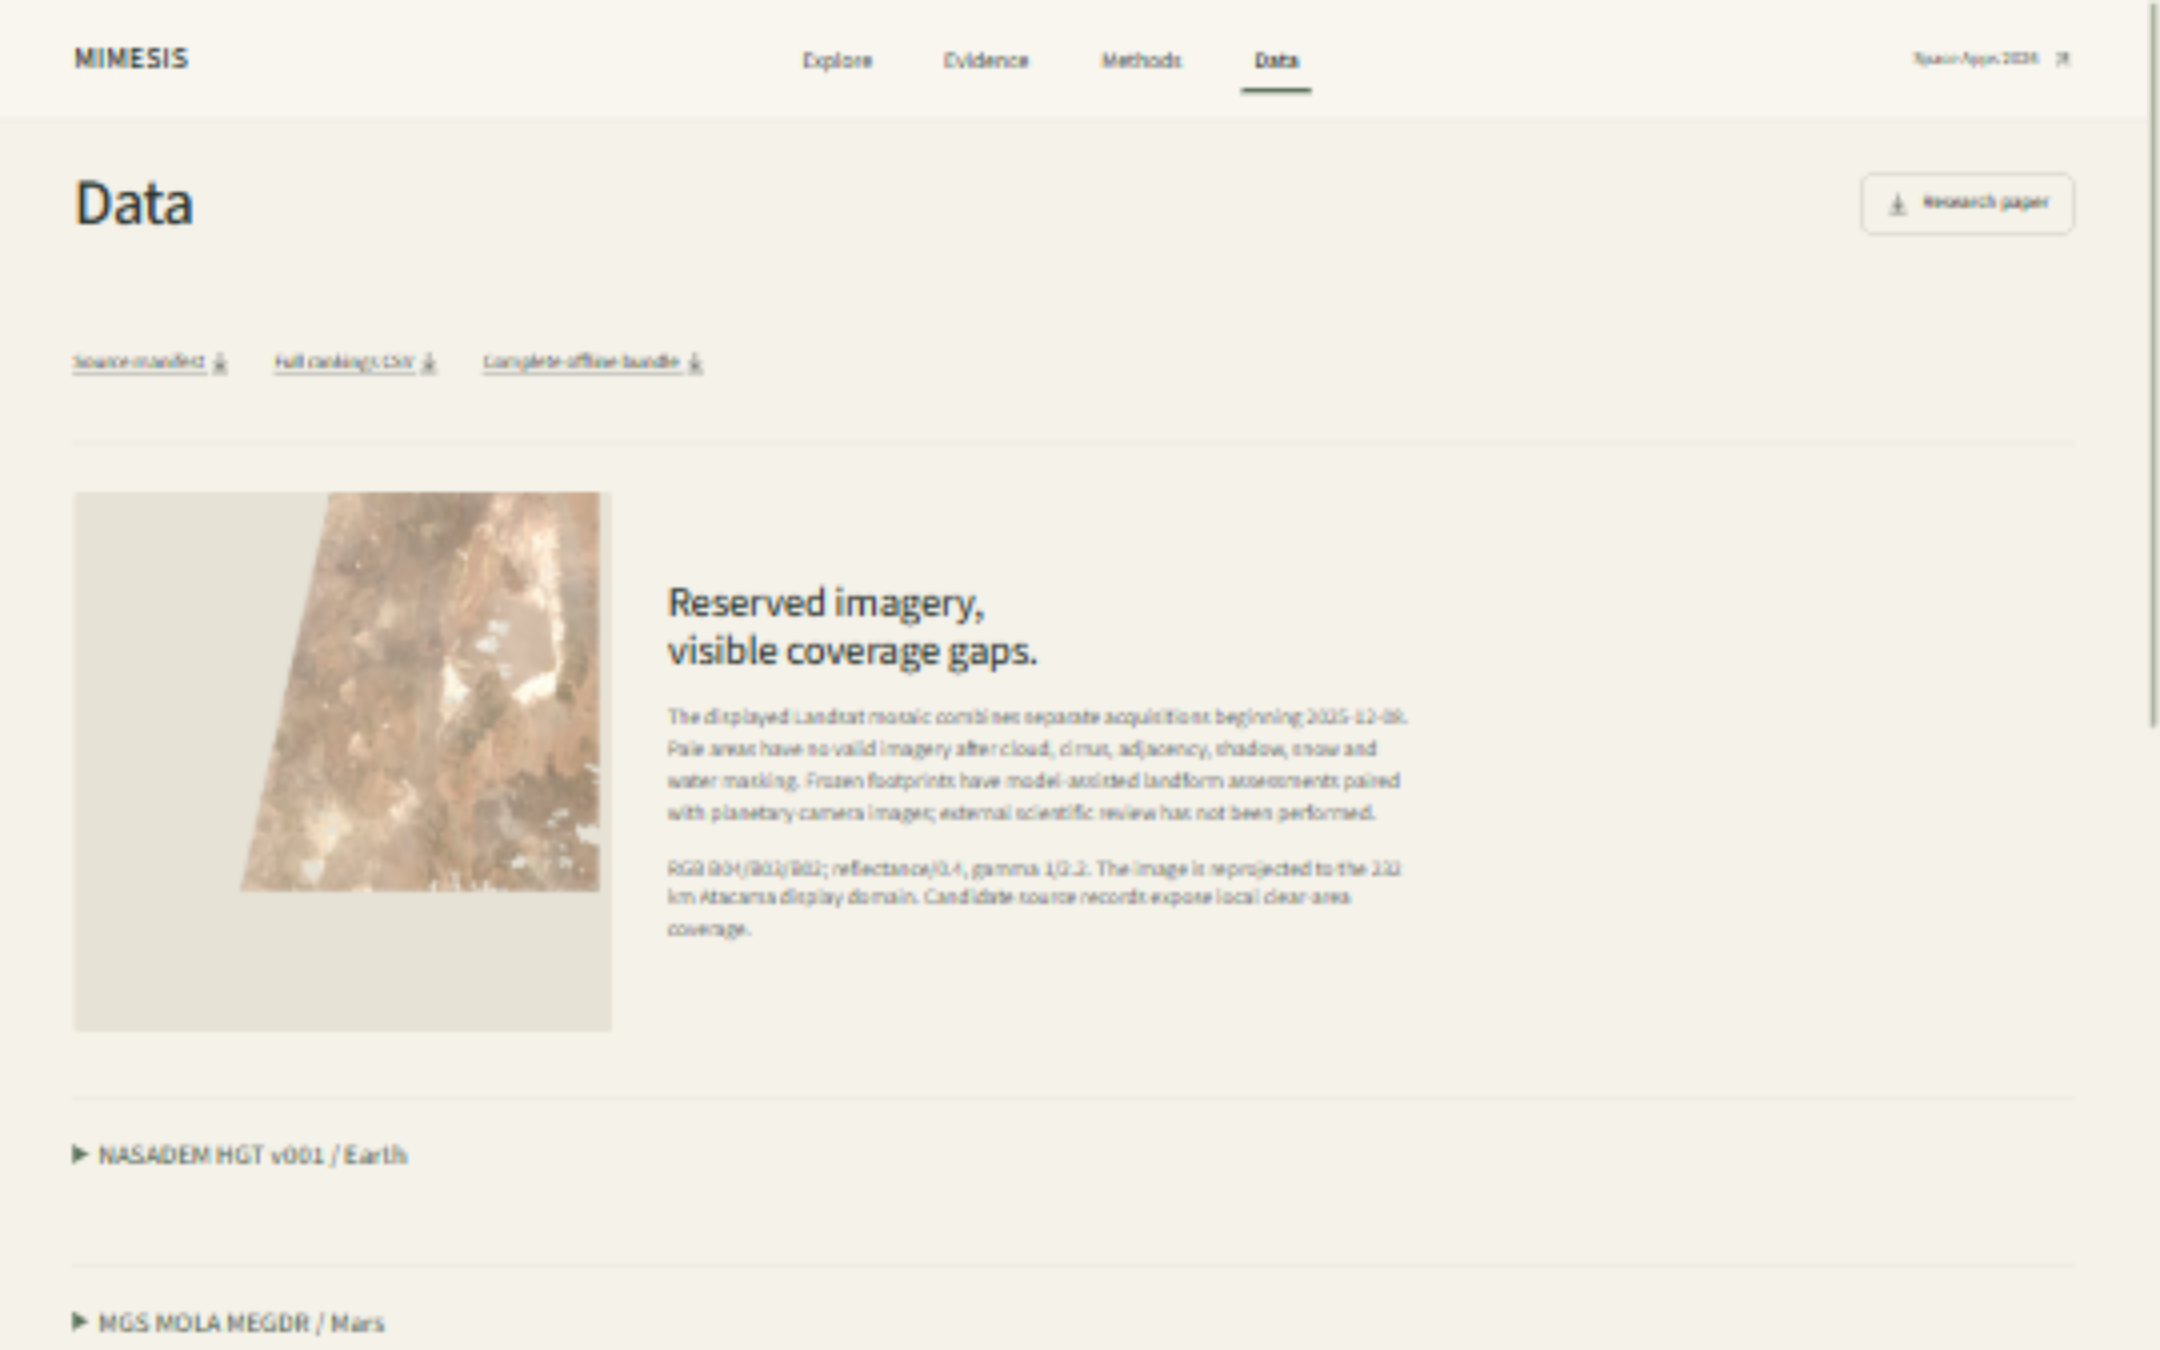
\includegraphics[width=\linewidth,height=104mm,keepaspectratio]{images/data.png}
\source{Observation sources, imagery gaps, manifests and full ranking exports.}
\end{column}
\end{columns}
\par\medskip
Shortlist rule: minimize the worse rank across supports.\par
GeoJSON retains footprints, source IDs and validation status.
\end{frame}

\begin{frame}{Failed source checks stop stronger scientific claims}
\begin{columns}[T,onlytextwidth]
\begin{column}{.60\textwidth}
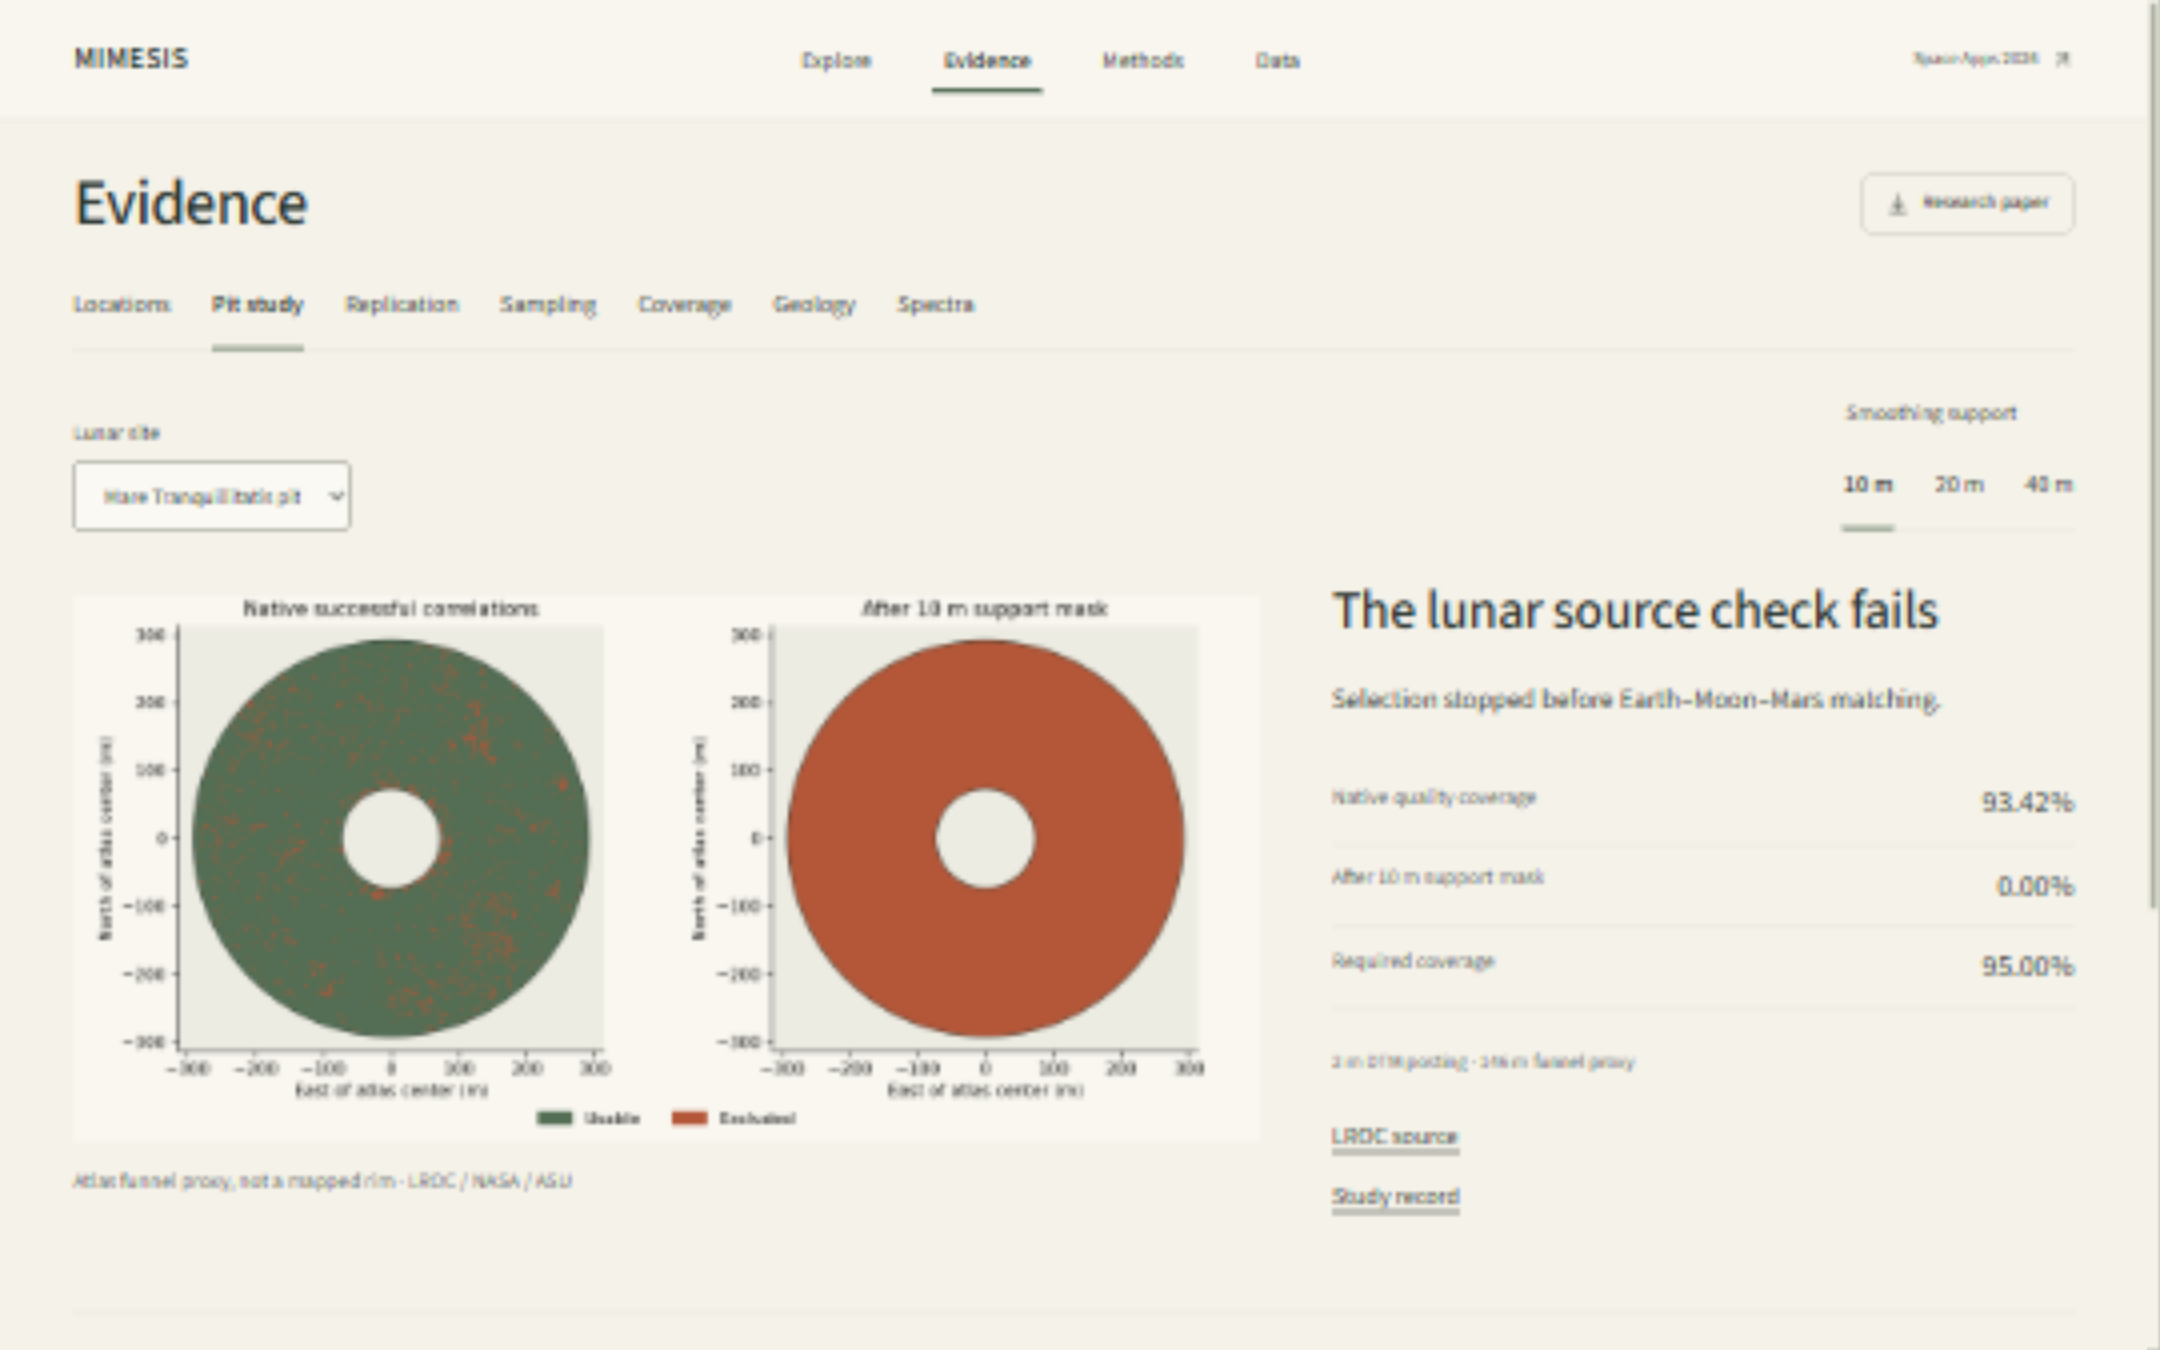
\includegraphics[width=\linewidth,height=120mm,keepaspectratio]{images/pit-study.png}
\source{Actual lunar calibration screen. An atlas proxy is not an independently mapped rim.}
\end{column}
\begin{column}{.37\textwidth}
\textbf{Lunar pit pilot}\par
At 10 m support: 0\% and 1.56\% usable exterior coverage versus 95\% required. All 120 mask sensitivities fail.
\par\medskip
\textbf{Sampling diagnostic}\par
All 18 MOLA-pattern transfers lower median Earth slope under the declared reconstruction.
\par\medskip
\textbf{Validity boundary}\par
Nine scientific/API tests and source hashes check software and evidence handling. They do not validate geology or field utility.
\end{column}
\end{columns}
\end{frame}

\begin{frame}{A working tool, a measured finding and a reproducible next step}
\begin{columns}[T,onlytextwidth]
\begin{column}{.48\textwidth}
\textbf{Contribution}\par
Separate rank turnover, shared ground and scoring-dependent geography before choosing an analogue.
\par\medskip
\textbf{A concrete follow-up window}\par
Nili scalar compromise: Namibia,\par
$25.16248^\circ$ S, $16.05951^\circ$ E.\par
Ranks 17 and 19; not a top-ten consensus.
\par\medskip
\textbf{Intended impact}\par
Help mapping teams choose what to investigate next. Mission savings and task benefit remain unmeasured.
\end{column}
\begin{column}{.48\textwidth}
\textbf{Delivered}\par
Four-view explorer; location GeoJSON; measured records; ten-page paper; two-page brief; editable Beamer deck.
\par\medskip
\textbf{Next scientific evidence}\par
Independent geological reference zones, qualified sources and outcomes for a declared exploration task.
\par\medskip
\textbf{Novelty boundary}\par
An original project-level geographic result. No newly validated geological analogue, safe base site or world-first method is claimed.
\end{column}
\end{columns}
\par\medskip
\href{https://github.com/ArjunCodess/MIMESIS}{github.com/ArjunCodess/MIMESIS}
\source{Built by Arjun Vijay Prakash; Codex assisted with implementation, analysis code and writing. Original source terms and research citations are retained.}
\end{frame}
\end{document}
